\subsection{Authors}

\begin{itemize}
    \item \href{https://github.com/BSoDium}{Philippe Négrel-Jerzy} (\href{mailto:negreljerzy.philippe@gmail.com}{negreljerzy.philippe@gmail.com})
    \item \href{https://github.com/seba1204}{Sébastien Pont} (\href{mailto:sepont@edu.aau.at}{sepont@edu.aau.at})
\end{itemize}

\subsection{Context}

This project is one of the assignments of the course \textit{Fundamental Topics in Multimedia Systems} at the \href{https://www.aau.at/en/}{Alpen-Adria-Universität Klagenfurt}.
The goal of this project is to implement a JPEG compression algorithm in Python.

\subsection{Project structure}


\dirtree{%
    .1 /.
    .2 assets.
    .3 tests.png.
    .3 head.jpg.
    .2 docs.
    .2 lib.
    .3 compressor.py.
    .3 decompressor.py.
    .3 dct.py.
    .3 run\_length\_encoding.py.
    .3 quantization.py.
    .3 zigzag.py.
    .2 out.
    .2 src.
    .2 main.py.
}


The program start with the \iCode{main} function in \iCode{main.py}.
It inits what is needed to run the program. You can call it with the following command:

\sFF{src/part-00/assets/command.txt}{Run Compressor}{run-command}

You can find all CLI options in Annex \ref{annex:cli-options} of this document
or \href{https://github.com/seba1204/jpeg-compressor/wiki}{here}.
The interesting part of the program is in the \iCode{lib} folder,
especially in the \iCode{compressor.py} file.

For test purposes, I used two images cropped :

\begin{figure}[H]
    \centering
    % subfigures 2 images
    \begin{subfigure}[b]{0.4\textwidth}
        \centering
        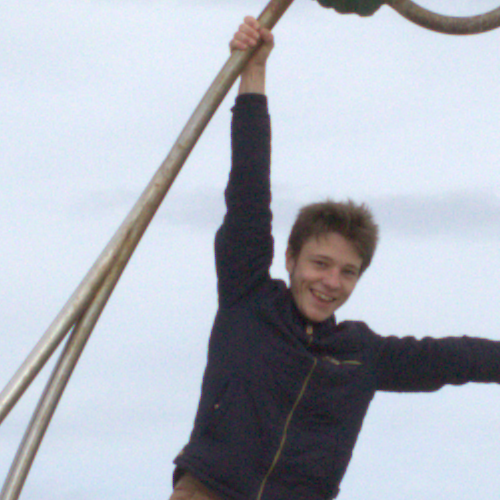
\includegraphics[width=0.4\textwidth]{src/assets/tests/tests.png}
        \caption{Tests image}
        \label{fig:tests}
    \end{subfigure}
    \begin{subfigure}[b]{0.4\textwidth}
        \centering
        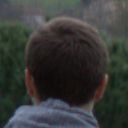
\includegraphics[width=0.4\textwidth]{src/assets/head/head.jpg}
        \caption{Head image}
        \label{fig:head}
    \end{subfigure}
\end{figure}

\subsection{References}

Here is a list of tutos that I used to implement this project:

\begin{dinglist}{111}
    \item \href{https://yasoob.me/posts/understanding-and-writing-jpeg-decoder-in-python}{Understanding and Decoding a JPEG Image using Python}
    \item \href{https://parametric.press/issue-01/unraveling-the-jpeg/}{Unraveling the JPEG}
    \item \href{https://youtu.be/JsTptu56GM8}{JPEG DCT, Discrete Cosine Transform (JPEG Pt2)- Computerphile}
    \item \href{https://youtu.be/Q2aEzeMDHMA}{How Computers Compress Text: Huffman Coding and Huffman Trees}
    \item \href{https://en.wikipedia.org/wiki/JPEG}{JPEG - Wikipedia}
    \item \href{https://www.sciencedirect.com/science/article/pii/S1742287608000285}{Using JPEG quantization tables}
\end{dinglist}
